\documentclass [10pt] {article}
\usepackage{amsmath,amsfonts,amsthm,amssymb}
\usepackage{fancyhdr}
\usepackage{fancyvrb}
\usepackage{textcomp}
\usepackage{listings,color}
\usepackage{verbatim}
\usepackage{chngpage}
\usepackage[pdftex]{graphicx}
\usepackage{color}
\usepackage{boxedminipage}
\usepackage{enumerate}
\usepackage{lineno}
\usepackage{color}
\usepackage[table]{xcolor}
\definecolor{lightgray}{rgb}{.9,.9,.9}
\definecolor{darkgray}{rgb}{.4,.4,.4}
\definecolor{purple}{rgb}{0.65, 0.12, 0.82}
\lstdefinelanguage{JavaScript}{
  keywords={break, case, catch, continue, debugger, default, delete, do, else, false, finally, for, function, if, in, instanceof, new, null, return, switch, this, throw, true, try, typeof, var, void, while, with},
  morecomment=[l]{//},
  morecomment=[s]{/*}{*/},
  morestring=[b]',
  morestring=[b]",
  ndkeywords={class, export, boolean, throw, implements, import, this},
  keywordstyle=\color{blue}\bfseries,
  ndkeywordstyle=\color{darkgray}\bfseries,
  identifierstyle=\color{black},
  commentstyle=\color{purple}\ttfamily,
  stringstyle=\color{red}\ttfamily,
  sensitive=true
}

\lstset{
   language=JavaScript,
   backgroundcolor=\color{lightgray},
   extendedchars=true,
   basicstyle=\footnotesize\ttfamily,
   showstringspaces=false,
   showspaces=false,
   numbers=left,
   numberstyle=\footnotesize,
   numbersep=9pt,
   tabsize=2,
   breaklines=true,
   showtabs=false,
   captionpos=b
}

\def\eolqed{\hspace{\stretch1}\ensuremath\qedsymbol}
\newcommand{\rpm}{\raisebox{.2ex}{$\scriptstyle\pm$}}
\setlength{\topmargin}{0in}
\setlength{\headheight}{0in}
\setlength{\headsep}{0in}
\setlength{\textheight}{7.7in}
\setlength{\textwidth}{6.5in}
\setlength{\oddsidemargin}{0in}
\setlength{\evensidemargin}{0in}
\setlength{\parindent}{0.25in}
\setlength{\parskip}{0.25in}

\lstset{
basicstyle=\footnotesize,
breaklines=true,
frame=single,
numbers=left,
keywordstyle=\color{blue},
stringstyle=\color{cyan},
commentstyle=\color{red},
language=Java,
showstringspaces=false,
tabsize=2
}

\title{CS 4153: Mobile App Development \newline
Homework 4}
\author{Scott Bushyhead}
\begin{document}

\begin{flushright}
{\huge  CS 4153: Mobile App Development}\\[5pt]
{\huge  Homework 4}\\[15pt]
\vspace{4pt}
\hrule
\vspace{4pt}
\hrule
{\large  Scott Bushyhead}\\[5pt]
{\large September 10, 2016}\\[5pt]
\end{flushright}

\newpage

% \begin{verbatim}
% \end{verbatim}
% \includegraphics[width=2.5in]{Full Path to File}


\section{For each teammate, get his/her name, telephone number (recommended, but not required), email address, and an address that can be used with Google Hangouts.}
\subsection{We have an excel spreadsheet created for this purpose and also added a second sheet that we will use to track tasks.}

\section{Using your cell phone, take a photo that includes all present members of your group except you.  (I.e., you should not be in the photo.)  If you do not have a phone with a working camera, borrow a teammate’s phone, take the photo, and have the teammate email it to you.When you submit the photo, caption it with the names of your team members, so that anyone who sees the photo and caption can determine who’s who.Since some team members are on different campuses, this means the other team members must gather around the monitor displaying the remote members so that all team members will be in the photo.}

\subsection{Team Orange: From left: Ammar Hassan, Tyler Weppler, Srivalli Kanchibotla}
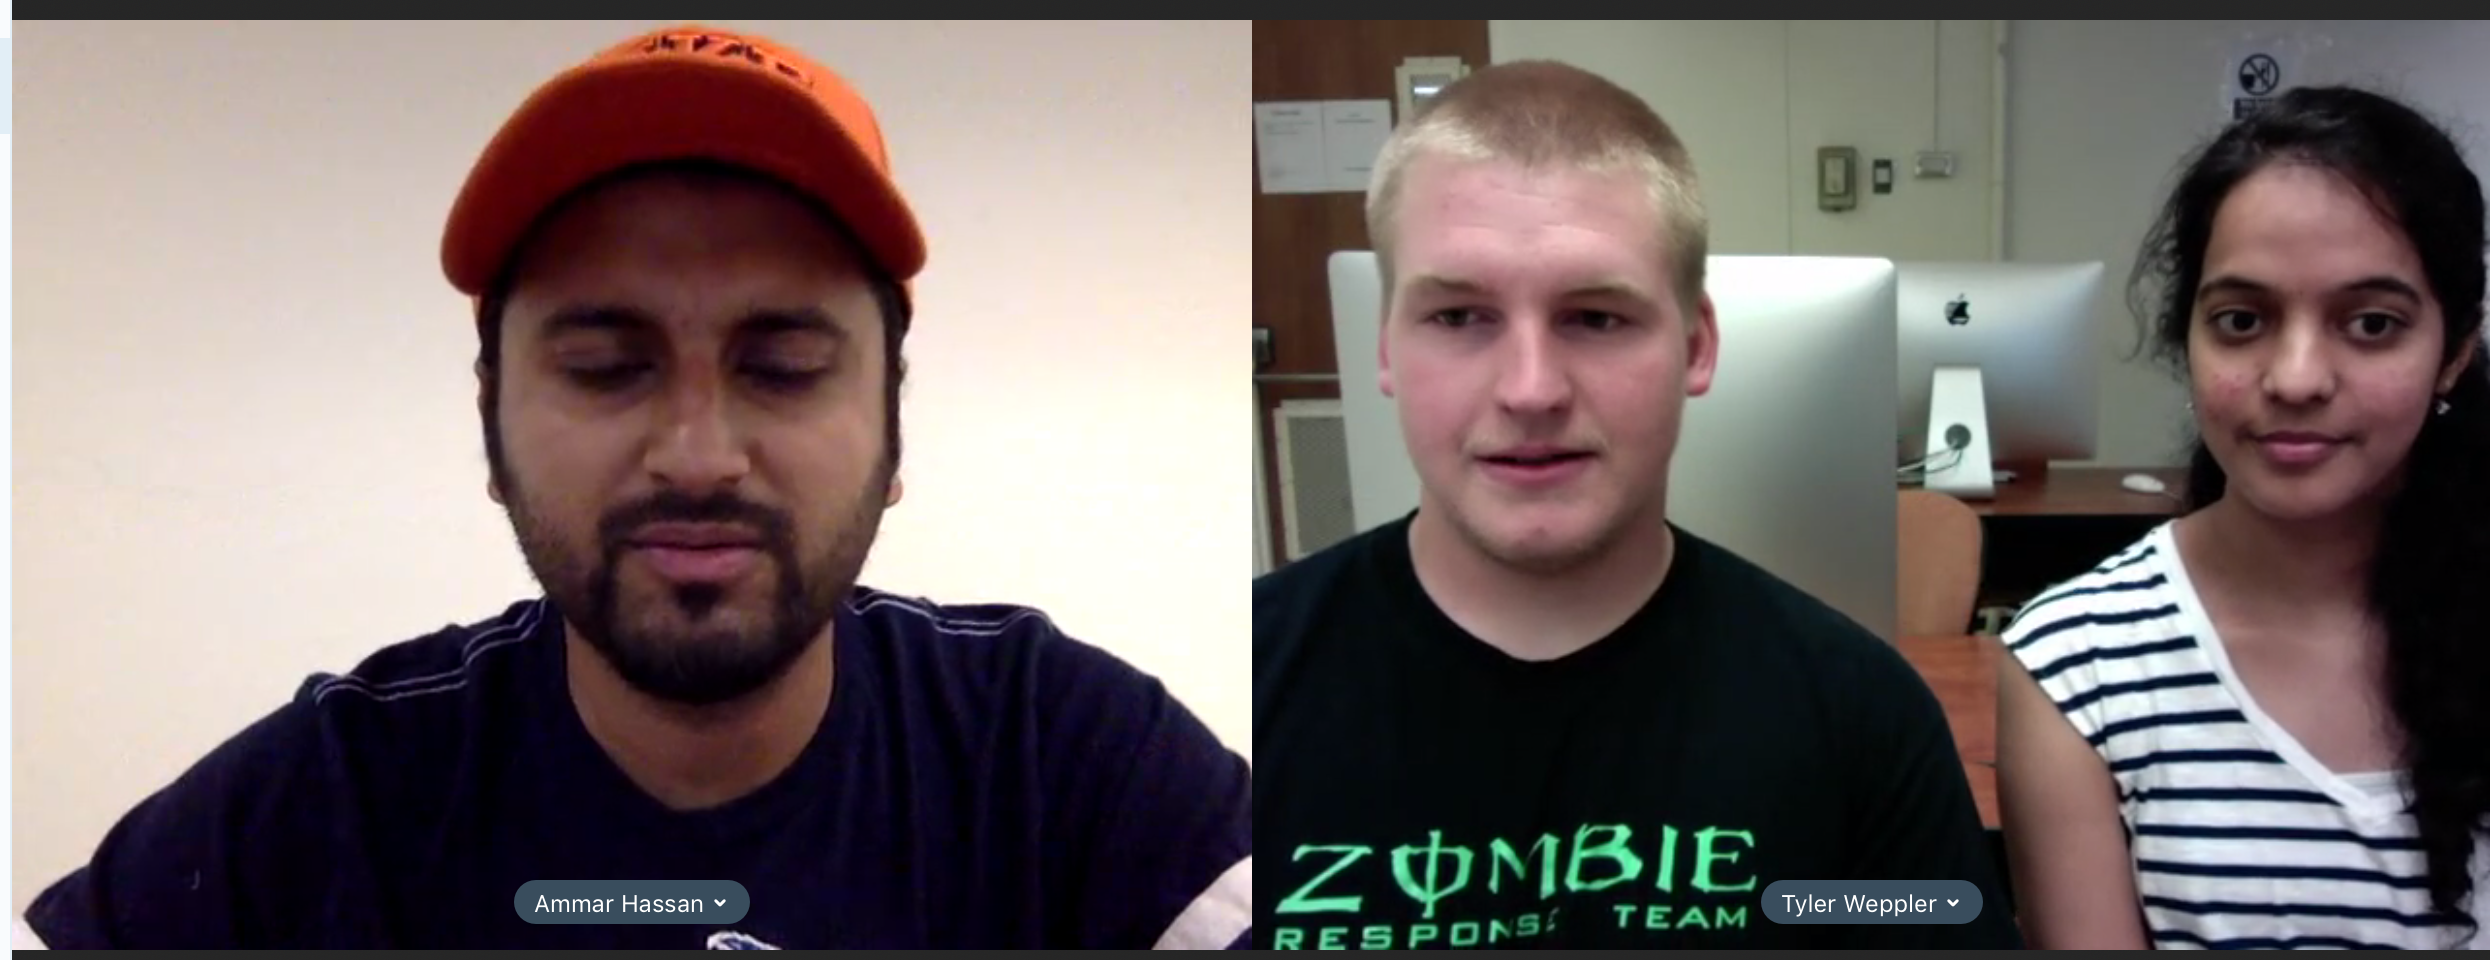
\includegraphics[width=2.5in]{Team_Orange.png}

\section{Find out why each of your teammates took the class and what they hope to get out of it (other than a good grade).}
\subsection{Tyler: Already enjoys programing for mobile, but wants to get better and specifically learn swift.}
\subsection{Srivalli: I want to learn app development design and develop an app of my own}
\subsection{Scott: I wanted to learn how to develop for mobile platforms and integrate with professional needs.}
\subsection{Ammar: I want to enhance my programming scope. Also want to learn app development.}

\section{Learn the favorite type of music for each of your teammates, and their favorite musical artist.}
\subsection{Tyler: Hard Rock/Metal/Some Rap. My favorite artist is Avenged Sevenfold.}
\subsection{Srivalli: Indian classic. Favorite Artist is Shankar mahadevan}
\subsection{Scott: Classic Rock.  Favorite Artist is Eric Clapton.}
\subsection{Ammar: Ambient / Electronica / Indian Music / Some Rock and Rap. Favorite artists are Enigma, A.R.Rahman, Buddha Bar, Nusrat Fateh Ali Khan.}

\section{As a team, choose one of the following mobile apps - Facebook}
\subsection{Strengths: 1. Strong APIs that allow it to be a part of many other apps. 2. Has the social networking foundation down to connect people. 3.Strong facial recognition}
\subsection{Weaknesses: 1. Security, or lack there of. 2. Separate app for messenger. 3. Exploiting its users (Negative Business Plan?)}
\subsection{Changes: 1. More customization of the parts, so the favorites/frequently used pieces could be all in in a single view. 2. Increased security with a possible team dedicated to protecting users and preventing crime.}


\section{Remarks}
\begin{enumerate}
\item Team Orange! Good group of workers, looking forward to this team project!
\end{enumerate}

Deadline: September 13, 2016

\end{document}

